% Options for packages loaded elsewhere
\PassOptionsToPackage{unicode}{hyperref}
\PassOptionsToPackage{hyphens}{url}
%
\documentclass[
]{article}
\usepackage{amsmath,amssymb}
\usepackage{lmodern}
\usepackage{iftex}
\ifPDFTeX
  \usepackage[T1]{fontenc}
  \usepackage[utf8]{inputenc}
  \usepackage{textcomp} % provide euro and other symbols
\else % if luatex or xetex
  \usepackage{unicode-math}
  \defaultfontfeatures{Scale=MatchLowercase}
  \defaultfontfeatures[\rmfamily]{Ligatures=TeX,Scale=1}
\fi
% Use upquote if available, for straight quotes in verbatim environments
\IfFileExists{upquote.sty}{\usepackage{upquote}}{}
\IfFileExists{microtype.sty}{% use microtype if available
  \usepackage[]{microtype}
  \UseMicrotypeSet[protrusion]{basicmath} % disable protrusion for tt fonts
}{}
\makeatletter
\@ifundefined{KOMAClassName}{% if non-KOMA class
  \IfFileExists{parskip.sty}{%
    \usepackage{parskip}
  }{% else
    \setlength{\parindent}{0pt}
    \setlength{\parskip}{6pt plus 2pt minus 1pt}}
}{% if KOMA class
  \KOMAoptions{parskip=half}}
\makeatother
\usepackage{xcolor}
\IfFileExists{xurl.sty}{\usepackage{xurl}}{} % add URL line breaks if available
\IfFileExists{bookmark.sty}{\usepackage{bookmark}}{\usepackage{hyperref}}
\hypersetup{
  hidelinks,
  pdfcreator={LaTeX via pandoc}}
\urlstyle{same} % disable monospaced font for URLs
\usepackage{color}
\usepackage{fancyvrb}
\newcommand{\VerbBar}{|}
\newcommand{\VERB}{\Verb[commandchars=\\\{\}]}
\DefineVerbatimEnvironment{Highlighting}{Verbatim}{commandchars=\\\{\}}
% Add ',fontsize=\small' for more characters per line
\newenvironment{Shaded}{}{}
\newcommand{\AlertTok}[1]{\textcolor[rgb]{1.00,0.00,0.00}{\textbf{#1}}}
\newcommand{\AnnotationTok}[1]{\textcolor[rgb]{0.38,0.63,0.69}{\textbf{\textit{#1}}}}
\newcommand{\AttributeTok}[1]{\textcolor[rgb]{0.49,0.56,0.16}{#1}}
\newcommand{\BaseNTok}[1]{\textcolor[rgb]{0.25,0.63,0.44}{#1}}
\newcommand{\BuiltInTok}[1]{#1}
\newcommand{\CharTok}[1]{\textcolor[rgb]{0.25,0.44,0.63}{#1}}
\newcommand{\CommentTok}[1]{\textcolor[rgb]{0.38,0.63,0.69}{\textit{#1}}}
\newcommand{\CommentVarTok}[1]{\textcolor[rgb]{0.38,0.63,0.69}{\textbf{\textit{#1}}}}
\newcommand{\ConstantTok}[1]{\textcolor[rgb]{0.53,0.00,0.00}{#1}}
\newcommand{\ControlFlowTok}[1]{\textcolor[rgb]{0.00,0.44,0.13}{\textbf{#1}}}
\newcommand{\DataTypeTok}[1]{\textcolor[rgb]{0.56,0.13,0.00}{#1}}
\newcommand{\DecValTok}[1]{\textcolor[rgb]{0.25,0.63,0.44}{#1}}
\newcommand{\DocumentationTok}[1]{\textcolor[rgb]{0.73,0.13,0.13}{\textit{#1}}}
\newcommand{\ErrorTok}[1]{\textcolor[rgb]{1.00,0.00,0.00}{\textbf{#1}}}
\newcommand{\ExtensionTok}[1]{#1}
\newcommand{\FloatTok}[1]{\textcolor[rgb]{0.25,0.63,0.44}{#1}}
\newcommand{\FunctionTok}[1]{\textcolor[rgb]{0.02,0.16,0.49}{#1}}
\newcommand{\ImportTok}[1]{#1}
\newcommand{\InformationTok}[1]{\textcolor[rgb]{0.38,0.63,0.69}{\textbf{\textit{#1}}}}
\newcommand{\KeywordTok}[1]{\textcolor[rgb]{0.00,0.44,0.13}{\textbf{#1}}}
\newcommand{\NormalTok}[1]{#1}
\newcommand{\OperatorTok}[1]{\textcolor[rgb]{0.40,0.40,0.40}{#1}}
\newcommand{\OtherTok}[1]{\textcolor[rgb]{0.00,0.44,0.13}{#1}}
\newcommand{\PreprocessorTok}[1]{\textcolor[rgb]{0.74,0.48,0.00}{#1}}
\newcommand{\RegionMarkerTok}[1]{#1}
\newcommand{\SpecialCharTok}[1]{\textcolor[rgb]{0.25,0.44,0.63}{#1}}
\newcommand{\SpecialStringTok}[1]{\textcolor[rgb]{0.73,0.40,0.53}{#1}}
\newcommand{\StringTok}[1]{\textcolor[rgb]{0.25,0.44,0.63}{#1}}
\newcommand{\VariableTok}[1]{\textcolor[rgb]{0.10,0.09,0.49}{#1}}
\newcommand{\VerbatimStringTok}[1]{\textcolor[rgb]{0.25,0.44,0.63}{#1}}
\newcommand{\WarningTok}[1]{\textcolor[rgb]{0.38,0.63,0.69}{\textbf{\textit{#1}}}}
\usepackage{graphicx}
\makeatletter
\def\maxwidth{\ifdim\Gin@nat@width>\linewidth\linewidth\else\Gin@nat@width\fi}
\def\maxheight{\ifdim\Gin@nat@height>\textheight\textheight\else\Gin@nat@height\fi}
\makeatother
% Scale images if necessary, so that they will not overflow the page
% margins by default, and it is still possible to overwrite the defaults
% using explicit options in \includegraphics[width, height, ...]{}
\setkeys{Gin}{width=\maxwidth,height=\maxheight,keepaspectratio}
% Set default figure placement to htbp
\makeatletter
\def\fps@figure{htbp}
\makeatother
\setlength{\emergencystretch}{3em} % prevent overfull lines
\providecommand{\tightlist}{%
  \setlength{\itemsep}{0pt}\setlength{\parskip}{0pt}}
\setcounter{secnumdepth}{-\maxdimen} % remove section numbering
\ifLuaTeX
  \usepackage{selnolig}  % disable illegal ligatures
\fi

\author{}
\date{}

\begin{document}

\hypertarget{homework-1-gradient-descent-and-convexity}{%
\section{Homework 1: Gradient Descent and
Convexity}\label{homework-1-gradient-descent-and-convexity}}

By Fernando Leal

\hypertarget{initial-definitions}{%
\subsubsection{Initial definitions}\label{initial-definitions}}

\begin{enumerate}
\def\labelenumi{\arabic{enumi}.}
\item
  \(x_i, \dots, x_m \in \mathbb{R}^{n\times n}, X\in\text{Mat}_{m \times n^2}(\mathbb{R})\)
\item
  \(\sigma(z) = \frac{1}{1+e^{-z}}\)
\item
  \(\theta = (x,b) \in \mathbb{R}^{n\times m}\times \mathbb{R}\)
\item
  \(\Pr(y_i \mid x_i, \theta) = \sigma(\left<x_i,x\right> + b)^{y_i}\sigma(-\left<x_i,x\right> - b)^{1-y_i}\)
\item
  \(\ell(\theta)=\prod_{i=1}^{m}\Pr(y_i\mid x_i,\theta)\)
\item
  \(f:\mathbb{R}^{n\times m + 1}\to\mathbb{R}:\theta\mapsto f(\theta) = -\log(\ell(\theta))\)
\item
  \(\tilde{x}_i = (x_i,1)\), a concatenation
\end{enumerate}

\hypertarget{question-1}{%
\subsubsection{Question 1}\label{question-1}}

\begin{quote}
Verify that

\[f(\theta) = 
\sum_{i=1}^{m}y_i\log(1+e^{-\left<\tilde{x}_i,\theta\right>}) + (1- y_i)\log(1+e^{\left<\tilde{x}_i, \theta\right>})\]
\end{quote}

\begin{align}
f(\theta) &= -\log(\ell(\theta)) =\\
&= -\log\left(\prod_{i=1}^{m}\Pr(y_i\mid x_i,\theta)\right) =\\
&= -\log\left(\prod_{i=1}^{m}\sigma(\left<\tilde{x}_i,\theta\right>)^{y_i}\sigma(-\left<\tilde{x}_i,\theta\right>)^{1-y_i}\right) =\\
&= -\sum_{i=1}^{m}\log\left(\sigma(\left<\tilde{x}_i,\theta\right>)^{y_i}\sigma(-\left<\tilde{x}_i,\theta\right>)^{1-y_i}\right) =\\
&=-\sum_{i=1}^{m}y_i\log\left(\sigma(\left<\tilde{x}_i,\theta\right>)\right) + (1-y_i)\log\left(\sigma(-\left<\tilde{x}_i,\theta\right>)\right) =\\
&=-\sum_{i=1}^{m}y_i\log\left((1+e^{\left<\tilde{x}_i,\theta\right>})^{-1}\right) + (1-y_i)\log\left((1+e^{-\left<\tilde{x}_i,\theta\right>})^{-1}\right) =\\
&= -\sum_{i=1}^{m}-y_i\log\left(1+e^{\left<\tilde{x}_i,\theta\right>}\right) - (1-y_i)\log\left(1+e^{-\left<\tilde{x}_i,\theta\right>}\right) =\\
&=\ \;\sum_{i=1}^{m}y_i\log\left(1+e^{\left<\tilde{x}_i,\theta\right>}\right) + (1-y_i)\log\left(1+e^{-\left<\tilde{x}_i,\theta\right>}\right)
\end{align}

\hypertarget{question-2}{%
\subsubsection{Question 2}\label{question-2}}

\begin{quote}
Show that \(z\mapsto \log(1+e^z)\) is convex
\end{quote}

Let \(g(z) := \log(1 + e^z)\), then \(g'(z) = \frac{e^z}{1+e^z}\) and
\(g''(z) = \frac{e^z(1+e^z) - e^z(e^z)}{(1+e^z)^2} = \frac{e^z}{(1+e^z)^2}\),
for which we see that \(\forall x\in\mathbb{R}, g''(z)\ge0\), and
therefore \(g\) is convex.

\hypertarget{question-3}{%
\subsubsection{Question 3}\label{question-3}}

\begin{quote}
Show that \(f\) is convex
\end{quote}

From \protect\hyperlink{question-1-1}{Question 1} we see that

\begin{align}
f(\theta) &= \sum_{i=1}^{m}y_i\log\left(1+e^{\left<\tilde{x}_i,\theta\right>}\right) + (1-y_i)\log\left(1+e^{-\left<\tilde{x}_i,\theta\right>}\right) =\\ 
&= \sum^m_{i=1}y_ig(\left<\tilde{x}_i,\theta\right>) + (1-y_i)g(-\left<\tilde{x}_i,\theta\right>)
\end{align}

which is but a non-negative weighted sum of a convex function \(g\)
composed with the affine mappings
\(\theta \mapsto \left<\tilde{x}_i,\theta\right>\) and
\(\theta \mapsto - \left<\tilde{x}_i,\theta\right>\). Since:

\begin{enumerate}
\def\labelenumi{\arabic{enumi}.}
\item
  Composing a convex function with an affine mapping preserves the
  convexity
\item
  Doing a non-negative weighted sum of convex functions preserves
  convexity
\end{enumerate}

Then we have that \(f\) is convex.

\hypertarget{question-4}{%
\subsubsection{Question 4}\label{question-4}}

\begin{quote}
Show that
\(f_\lambda(\theta) := f(\theta) + \frac{\lambda}{2}\lVert \theta \rVert^2\)
is strongly convex
\end{quote}

\(f_\lambda(\theta)\) is \(\mu\)-strongly convex if
\(f_\lambda(\theta) - \frac{\mu}{2}\lVert \theta \rVert ^2\) is convex.
If we choose \(\mu = \lambda\), by the definition of \(f_\lambda\) we
have

\[f_\lambda(\theta) - \frac{\lambda}{2}\lVert\theta\rVert^2 = f(\theta) - \frac{\lambda}{2}\lVert\theta\rVert^2 + \frac{\lambda}{2}\lVert\theta\rVert^2 = f(\theta)\]

which we already know is convex from
\protect\hyperlink{question-3-3}{Question 3}

\hypertarget{question-5}{%
\subsubsection{Question 5}\label{question-5}}

\begin{quote}
With \(\lambda  > 0\) argue that \(f_\lambda\) has a single global
minimum \(\theta \in \mathcal{E}\) for which
\(\nabla f_\lambda(\theta) = 0\)
\end{quote}

If \(\lambda > 0\), we've seen that \(f_\lambda\) is strongly convex in
\protect\hyperlink{question-4-4}{Question 4}, which means that it must
have a global minimum THEOREM\_REF, and that such minimum must be a
\(\theta\in\mathcal{E}\) where \(\nabla f_\lambda(\theta) = 0\).

An equivalent condition for \(f\) to be strongly convex with parameter
\(\lambda  > 0\) is that for \(x,y\)

\[f(y) \ge f(x) + \left<\nabla  f(x), x-y\right> + \frac{\lambda}{2}\lVert  x -y\rVert^2\]

With this condition, it's easy to see that given
\(\theta\in\mathbb{R}:\nabla  f(\theta) = 0\), then

\[f(\theta) \le f(y) - \frac{\lambda}{2}\lVert \theta      -y\rVert^2 \le f(y)\]

for all \(y\in\mathbb{R}\), which makes it a global maximum.

Also, if we had \(\theta_1, \theta_2\) such that
\(\nabla f(\theta_i) = 0\) for \(i\in\{1,2\}\), then
\(f(\theta_1) = f(\theta_2)\), but

\[f(\theta_2) = f(\theta_1) \le f(\theta_2) - \frac{\lambda}{2}\lVert  \theta_1  - \theta_2 \rVert^2 \iff \frac{\lambda}{2}\lVert \theta_1   - \theta_2 \rVert^2 = 0 \iff \theta_1 = \theta_2\]

which means that such a \(\theta\) is unique.

\hypertarget{question-6}{%
\subsubsection{Question 6}\label{question-6}}

\begin{quote}
Give an expression for \(\nabla f_\lambda\)
\end{quote}

By using the definition of
\(f_\lambda(x) = f(x) + \frac{\lambda}{2}\lVert x\rVert^2\) and
\(f(x) = \sum^{m}_{i=1}y_ig(\left<x_i,x\right>)) +  (1-y_i)g(-\left<x_i,x\right>)\),
and the simple facts:

\begin{enumerate}
\def\labelenumi{\arabic{enumi}.}
\item
  \(\nabla_x \lVert x \rVert^2 = 2x\)
\item
  \(\nabla_x\left<a,x\right>  = a\)
\end{enumerate}

We have that

\begin{align}
g'(x) &= (\log(1+e^x))' = \frac{e^x}{1+e^x} =\\
&= 1 - \frac{1}{1+e^x} \\
g'(-x) &= \frac{\frac{1}{e^x}}{1+\frac{1}{e^x}} = \frac{1}{e^x + 1} =\\
&= 1-g'(x) \\
\\

\nabla f(x) &= \sum^m_{i=1}
y_i\tilde{x_i}\nabla g(\left<\tilde{x_i},x\right>) -
(1-y_i)\tilde{x_i}\nabla g(-\left<\tilde{x_i},x\right>) =\\
&= \sum^m_{i=1}
\tilde{x_i}\left(y_i\nabla g(\left<\tilde{x_i},x\right>) -
(1-y_i)\nabla g(-\left<\tilde{x_i},x\right>) \right) =\\
&= \sum^m_{i=1}
\tilde{x_i}\left(y_i\left( 1 - \nabla g(-\left<\tilde{x_i},x\right>)\right) -
(1-y_i)\nabla g(-\left<\tilde{x_i},x\right>) \right) =\\
&= \sum^m_{i=1}
\tilde{x_i}\left(y_i - y_i\nabla g(-\left<\tilde{x_i},x\right>) -
\nabla g(-\left<\tilde{x_i},x\right>) + y_i\nabla g(-\left<\tilde{x_i},x\right>) \right) =\\
&= \sum^m_{i=1}
\tilde{x_i}\left(y_i -
\nabla g(-\left<\tilde{x_i},x\right>)\right) \\
\\

\nabla f_\lambda(x) &= \nabla f(x) + \nabla (\frac{\lambda}{2}\lVert x\rVert^2) =\\
&= \nabla f(x) + \lambda x =\\
&= \sum^m_{i=1}
\tilde{x_i}\left(y_i -
\nabla g(-\left<\tilde{x_i},x\right>)\right) + \lambda x
\\
\end{align}

\hypertarget{question-7}{%
\subsubsection{Question 7}\label{question-7}}

\begin{quote}
Implement a function
\texttt{{[}f,g{]}\ =\ logistic\_regression(train,\ \ theta,\ lambda)}
that takes as input the training data \(\theta\in\mathcal{E}\) and
returns the output value \(f_\lambda(\theta)\) and the gradient
\(\nabla f_\lambda(\theta)\) for some fixed \(\lambda\)
\end{quote}

\begin{Shaded}
\begin{Highlighting}[]
\KeywordTok{function}\NormalTok{ [}\VariableTok{f}\OperatorTok{,}\VariableTok{g}\NormalTok{] }\OperatorTok{=} \VariableTok{logistic\_regression}\NormalTok{(}\VariableTok{train}\OperatorTok{,} \VariableTok{theta}\OperatorTok{,} \VariableTok{lambda}\NormalTok{)}
    \VariableTok{X} \OperatorTok{=} \VariableTok{train}\NormalTok{.}\VariableTok{X}\OperatorTok{;}
    \VariableTok{y} \OperatorTok{=} \VariableTok{train}\NormalTok{.}\VariableTok{y}\OperatorTok{;}

    \VariableTok{cross\_product} \OperatorTok{=} \VariableTok{X}\OperatorTok{\textquotesingle{}} \OperatorTok{*} \VariableTok{theta}\OperatorTok{;}
    \VariableTok{log\_\_} \OperatorTok{=} \VariableTok{log}\NormalTok{(}\FloatTok{1} \OperatorTok{+} \VariableTok{exp}\NormalTok{(}\VariableTok{sign}\NormalTok{(}\VariableTok{y}\NormalTok{) }\OperatorTok{.*} \VariableTok{cross\_product}\NormalTok{))}\OperatorTok{;}
    \VariableTok{f} \OperatorTok{=} \VariableTok{y} \OperatorTok{.*} \VariableTok{log\_\_} \OperatorTok{+}\NormalTok{ (}\FloatTok{1}\NormalTok{.}\OperatorTok{{-}}\VariableTok{y}\NormalTok{) }\OperatorTok{.*} \VariableTok{log\_\_}\OperatorTok{;}
    
    \VariableTok{exp\_\_} \OperatorTok{=} \VariableTok{exp}\NormalTok{(}\VariableTok{cross\_product}\NormalTok{)}\OperatorTok{;}
    \VariableTok{g} \OperatorTok{=} \VariableTok{lambda}\OperatorTok{*}\VariableTok{theta}  \OperatorTok{+} \VariableTok{X} \OperatorTok{*}\NormalTok{(}\VariableTok{exp\_\_} \OperatorTok{./}\NormalTok{ (}\FloatTok{1} \OperatorTok{+} \VariableTok{exp\_\_}\NormalTok{))}\OperatorTok{;}	
\KeywordTok{end}
\end{Highlighting}
\end{Shaded}

\hypertarget{question-8}{%
\subsubsection{Question 8}\label{question-8}}

\begin{quote}
Check that your gradient code is correct by generating a random
\(\theta\) nd \(v\) and ploting the error
\(\mid f_\lambda(\theta+tv)-f_\lambda(\theta) - t\left<v,\nabla f_\lambda(\theta)\right>\mid\)
versus \(t\) where \texttt{t\ =\ logspace(-8,0,101)}.
\end{quote}

\begin{Shaded}
\begin{Highlighting}[]
\KeywordTok{function} \VariableTok{checkgradient}\NormalTok{(}\VariableTok{fhandle}\OperatorTok{,} \VariableTok{theta}\OperatorTok{,} \VariableTok{v}\NormalTok{)    }
    \VariableTok{n} \OperatorTok{=} \FloatTok{101}\OperatorTok{;}
    \VariableTok{ts} \OperatorTok{=} \VariableTok{logspace}\NormalTok{(}\OperatorTok{{-}}\FloatTok{8}\OperatorTok{,} \FloatTok{0}\OperatorTok{,} \VariableTok{n}\NormalTok{)}\OperatorTok{;}
    
    \VariableTok{f\_theta\_tv} \OperatorTok{=} \VariableTok{fhandle}\NormalTok{(}\VariableTok{theta} \OperatorTok{+} \VariableTok{v}\OperatorTok{*}\VariableTok{ts}\NormalTok{)}\OperatorTok{;}
\NormalTok{    [}\VariableTok{f\_theta}\OperatorTok{,} \VariableTok{grad\_f\_theta}\NormalTok{] }\OperatorTok{=} \VariableTok{fhandle}\NormalTok{(}\VariableTok{theta}\NormalTok{)}\OperatorTok{;}

    \VariableTok{errors} \OperatorTok{=} \VariableTok{abs}\NormalTok{(}\VariableTok{f\_theta\_tv} \OperatorTok{{-}} \VariableTok{f\_theta} \OperatorTok{{-}}\NormalTok{ (}\VariableTok{v}\OperatorTok{\textquotesingle{}} \OperatorTok{*}\VariableTok{grad\_f\_theta}\NormalTok{)}\OperatorTok{*}\VariableTok{ts}\NormalTok{)}\OperatorTok{;}
    \VariableTok{loglog}\NormalTok{(}\VariableTok{ts}\OperatorTok{,} \VariableTok{errors}\NormalTok{)}
\KeywordTok{end}
\end{Highlighting}
\end{Shaded}

\hypertarget{question-9}{%
\subsubsection{Question 9}\label{question-9}}

\begin{quote}
What is the value of \(\frac{1}{4}\sigma_{\max}(X)^2\) for the training
set?
\end{quote}

\texttt{L\ =\ max(max(train.X))\^{}2/4}, which for our dataset turns out
to be \(21.0828\)

\hypertarget{question-10}{%
\subsubsection{Question 10}\label{question-10}}

\begin{quote}
Implement gradient descent with constant step-length \(\frac{1}{L}\) to
generate a sequence \(\theta_0 , \theta_1 , \theta_2 , \dots\)starting
from a random initial point \(\theta_0 \in E\) and with
\(\lambda = 10^{−4}\). The function should (at least) return the final
iterate, and the gradient norm and total running time at each iterate.
To measure time you can use the commands \texttt{tic} and \texttt{toc}.
\end{quote}

\begin{Shaded}
\begin{Highlighting}[]
\KeywordTok{function}\NormalTok{ [}\VariableTok{theta}\OperatorTok{,} \VariableTok{gradnorms}\OperatorTok{,} \VariableTok{times}\NormalTok{] }\OperatorTok{=} \VariableTok{cstgradientdescent}\NormalTok{(}\VariableTok{fhandle}\OperatorTok{,} \VariableTok{x0}\OperatorTok{,} \VariableTok{alpha}\OperatorTok{,} \VariableTok{params}\NormalTok{)}
    \VariableTok{maxiters} \OperatorTok{=} \VariableTok{params}\NormalTok{.}\VariableTok{maxiters}\OperatorTok{;}
    \VariableTok{maxtime} \OperatorTok{=} \VariableTok{params}\NormalTok{.}\VariableTok{maxtime}\OperatorTok{;}
    \VariableTok{tolgradnorm} \OperatorTok{=} \VariableTok{params}\NormalTok{.}\VariableTok{tolgradnorm}\OperatorTok{;}
    
    \VariableTok{gradnorms} \OperatorTok{=} \VariableTok{zeros}\NormalTok{(}\FloatTok{1}\OperatorTok{,} \VariableTok{maxiters} \OperatorTok{+} \FloatTok{1}\NormalTok{)}\OperatorTok{;}
    \VariableTok{times} \OperatorTok{=} \VariableTok{zeros}\NormalTok{(}\FloatTok{1}\OperatorTok{,} \VariableTok{maxiters} \OperatorTok{+} \FloatTok{1}\NormalTok{)}\OperatorTok{;}

    \VariableTok{xk} \OperatorTok{=} \VariableTok{x0}\OperatorTok{;}
    \VariableTok{tic}
    \KeywordTok{for} \VariableTok{iter} \OperatorTok{=} \FloatTok{1}\OperatorTok{:}\VariableTok{maxiters}
\NormalTok{        [}\OperatorTok{\textasciitilde{},} \VariableTok{max\_direction}\NormalTok{] }\OperatorTok{=} \VariableTok{fhandle}\NormalTok{(}\VariableTok{xk}\NormalTok{)}\OperatorTok{;}
        \VariableTok{min\_direction} \OperatorTok{=} \OperatorTok{{-}}\VariableTok{max\_direction}\OperatorTok{;}
        \VariableTok{xk} \OperatorTok{=} \VariableTok{xk} \OperatorTok{+} \VariableTok{alpha}\OperatorTok{*}\VariableTok{min\_direction}\OperatorTok{;}
        
        \VariableTok{times}\NormalTok{(}\VariableTok{iter}\NormalTok{) }\OperatorTok{=} \VariableTok{toc}\OperatorTok{;}
        \KeywordTok{if} \VariableTok{times}\NormalTok{(}\VariableTok{iter}\NormalTok{) }\OperatorTok{\textgreater{}} \VariableTok{maxtime}
            \KeywordTok{break}
        \KeywordTok{end}

        \VariableTok{gradnorms}\NormalTok{(}\VariableTok{iter}\NormalTok{) }\OperatorTok{=} \VariableTok{norm}\NormalTok{(}\VariableTok{min\_direction}\NormalTok{)}\OperatorTok{;}
        \KeywordTok{if} \VariableTok{gradnorms}\NormalTok{(}\VariableTok{iter}\NormalTok{) }\OperatorTok{\textless{}} \VariableTok{tolgradnorm}
            \KeywordTok{break}
        \KeywordTok{end}
        \KeywordTok{if} \VariableTok{gradnorms}\NormalTok{(}\VariableTok{iter}\NormalTok{) }\OperatorTok{/} \VariableTok{gradnorms}\NormalTok{(}\FloatTok{1}\NormalTok{) }\OperatorTok{\textless{}} \FloatTok{5e{-}4}
            \KeywordTok{break}
        \KeywordTok{end}
    \KeywordTok{end}
    
    \VariableTok{theta} \OperatorTok{=} \VariableTok{xk}\OperatorTok{;}
    \VariableTok{gradnorms} \OperatorTok{=} \VariableTok{gradnorms}\NormalTok{(}\FloatTok{1}\OperatorTok{:}\VariableTok{iter}\NormalTok{)}\OperatorTok{;}
    \VariableTok{times} \OperatorTok{=} \VariableTok{times}\NormalTok{(}\FloatTok{1}\OperatorTok{:}\VariableTok{iter}\NormalTok{)}\OperatorTok{;}
\KeywordTok{end}
\end{Highlighting}
\end{Shaded}

\hypertarget{question-11}{%
\subsubsection{Question 11}\label{question-11}}

\begin{quote}
Run the algorithm for at most 3 minutes, and show a plot of the norm of
the gradient \(\lVert\nabla f_\lambda (\theta_k)\rVert\) as a function
of \(k\) (log-scale on the vertical axis). You may include a stopping
criterion so that the algorithm stops whenever the ratio
\(\frac{\lVert\nabla  f_\lambda (\theta_k )\rVert}{\lVert\nabla f_\lambda(\theta_0)\rVert}\)
drops below a threshold \(\varepsilon\), for example
\(\varepsilon = 5 · 10^{−4}\)
\end{quote}

\begin{figure}
\centering
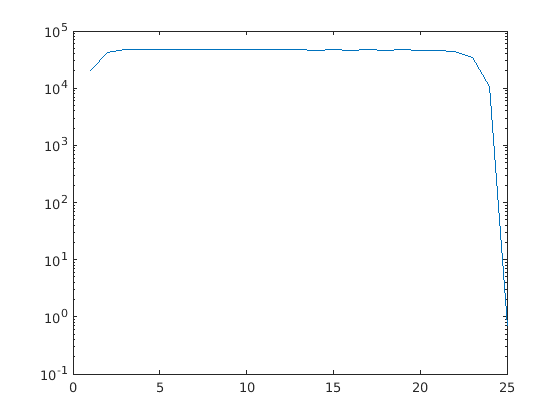
\includegraphics{/home/ayhon/uni/NO Nonlinear Optimization/gradient_norm_to_iterations.png}
\caption{}
\end{figure}

\hypertarget{question-12}{%
\subsubsection{Question 12}\label{question-12}}

\begin{quote}
Using properties of \(f_\lambda\) established here, and referring to
appropriate results in the lecture notes, argue that the algorithm
converges to the global minimizer of \(f_\lambda\). Be precise. Comment
briefly in light of the plot you produced in the previous question.
\end{quote}

Since \(f_\lambda\) is strongly convex, it's in particular convex, and
convex functions must have at most one global minimizer. Since it's also
strongly convex, we know that there must exist one global minimizer, and
that this minimizer is the \(\theta\in\mathcal{E}\) where
\(\nabla f_\lambda(\theta) =0\). As we see in the previous graph, our
function's norm approaches zero as the iterations go by, which tells us
we've hit the minimizer.

\hypertarget{question-13}{%
\subsubsection{Question 13}\label{question-13}}

\begin{quote}
Implement a backtracking line-search method (Algorithm 3.1 in Nocedal
and Wright) and run the same experiment as in question. You will have to
play around with parameters ᾱ, ρ, c. Typical values are ρ ∈ {[}0.5,
0.8{]} and c = 10−4 . For ᾱ, you can set a fixed value (tuned through
experimentation), or you can take inspiration from §3.5 in Nocedal and
Wright for fancier techniques where ᾱ changes with k. Show the new plot
of \(\lVert\nabla  f_\lambda (\theta_k )\rVert\) versus \(k\).
\end{quote}

\begin{Shaded}
\begin{Highlighting}[]
\KeywordTok{function} \VariableTok{alpha} \OperatorTok{=} \VariableTok{linesearch}\NormalTok{(}\VariableTok{fhandle}\OperatorTok{,} \VariableTok{x}\OperatorTok{,} \VariableTok{v}\OperatorTok{,} \VariableTok{lsparams}\NormalTok{)}
    \VariableTok{alphabar} \OperatorTok{=} \VariableTok{lsparams}\NormalTok{.}\VariableTok{alphabar}\OperatorTok{;}
    \VariableTok{c} \OperatorTok{=} \VariableTok{lsparams}\NormalTok{.}\VariableTok{c}\OperatorTok{;}
    \VariableTok{rho} \OperatorTok{=} \VariableTok{lsparams}\NormalTok{.}\VariableTok{rho}\OperatorTok{;}
    \VariableTok{alphamin} \OperatorTok{=} \VariableTok{lsparams}\NormalTok{.}\VariableTok{alphamin}\OperatorTok{;}
    
    \VariableTok{alpha} \OperatorTok{=} \VariableTok{alphabar}\OperatorTok{;}

\NormalTok{    [}\VariableTok{f\_x}\OperatorTok{,} \VariableTok{g\_f\_k}\NormalTok{] }\OperatorTok{=} \VariableTok{fhandle}\NormalTok{(}\VariableTok{x}\NormalTok{)}\OperatorTok{;}

    \KeywordTok{while} \VariableTok{alpha} \OperatorTok{\textgreater{}=} \VariableTok{alphamin}
        \KeywordTok{if} \VariableTok{fhandle}\NormalTok{(}\VariableTok{x} \OperatorTok{+} \VariableTok{alpha}\OperatorTok{*}\VariableTok{v}\NormalTok{) }\OperatorTok{\textless{}=} \VariableTok{f\_x} \OperatorTok{+} \VariableTok{c}\OperatorTok{*}\VariableTok{alpha}\OperatorTok{*}\NormalTok{(}\VariableTok{g\_f\_k}\OperatorTok{\textquotesingle{}*}\VariableTok{v}\NormalTok{)}
            \KeywordTok{break}
        \KeywordTok{end}
        \VariableTok{alpha} \OperatorTok{=} \VariableTok{rho} \OperatorTok{*} \VariableTok{alpha}\OperatorTok{;}
    \KeywordTok{end}
    
    \KeywordTok{if}\NormalTok{(}\VariableTok{rho} \OperatorTok{*} \VariableTok{alpha} \OperatorTok{\textless{}} \VariableTok{alphamin}\NormalTok{)}
        \VariableTok{warning}\NormalTok{(}\SpecialStringTok{\textquotesingle{}Backtracking minimum step size reached!\textquotesingle{}}\NormalTok{)}\OperatorTok{;}
    \KeywordTok{end}
\KeywordTok{end}
\end{Highlighting}
\end{Shaded}

\hypertarget{question-14}{%
\subsubsection{Question 14}\label{question-14}}

\begin{quote}
It is deceiving to compare the plots from questions 11 and 13, because
it hides the extra work that the line-search method had to do. On a
single plot, show the behavior of both algorithms, but this time with
\(\lVert\nabla  f_\lambda (\theta_k )\rVert\) (still on a log-scale)
versus computation time.
\end{quote}

\hypertarget{question-15}{%
\subsubsection{Question 15}\label{question-15}}

\begin{quote}
The θ you found through optimization is a pair θ = (x, b) ∈ Rn×n × R. In
particular, x is an image of the same size as the images in our data
set. Show this image in a grayscale figure (with a colorbar for scale)
and report the value of b.
\end{quote}

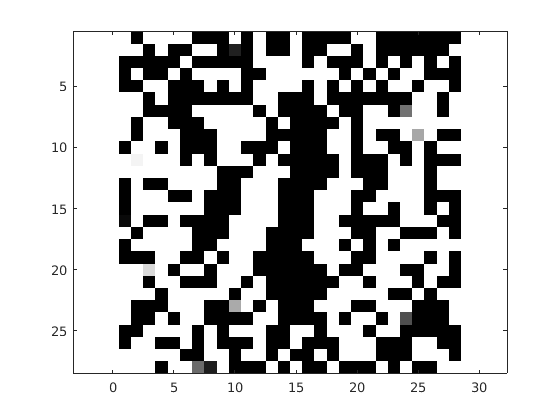
\includegraphics{/home/ayhon/uni/NO Nonlinear Optimization/new_image.png}

where \(b = -6.6611e+03\)

\hypertarget{question-16}{%
\subsubsection{Question 16}\label{question-16}}

\begin{quote}
For each image--label pair in the test set, \((x_i, y_i)\), compute
\(z_i = \sigma(h_\theta, \tilde{x}_i i)\) (again with
\(\tilde{x}_i = (x_i , 1)\)). If \(z_i > \frac{1}{2}\), you predict that
\(y_i = 1\), otherwise you predict \(y_i = 0\). Compare with the true
label \(y_i\) . Count the number of mistakes you make and report this
number (Matlab starter code: \texttt{binary\_classifier\_accuracy}).
Display the images that your \(\theta\) got wrong (Matlab starter code:
\texttt{showMNISTImages\_many}) and report the value of \(z_i\) for each
mistake (\(z_i\) is an indication of how confident your algorithm is.)
Do the same with the train data. Comment briefly with respect to our
overarching goal.
\end{quote}

\begin{figure}
\centering
\includegraphics{/home/ayhon/.var/app/io.typora.Typora/config/Typora/typora-user-images/image-20220315151420902.png}
\caption{}
\end{figure}

\begin{figure}
\centering
\includegraphics{/home/ayhon/.var/app/io.typora.Typora/config/Typora/typora-user-images/image-20220315151447618.png}
\caption{}
\end{figure}

\end{document}
